\mychapter{Vectors en el pla}{Vectors}{
\includegraphics[width=4cm]{img-08/wrhamilton}

{\small William Rowan Hamilton, 
	\par matemàtic Irlandès (1805-1865)}
}{chap:vectors}

\begin{blueshaded}
	Les diferents magnituds en la naturalesa es classifiquen en escalars i vectorials. Una magnitud és vectorial si depèn de la direcció.
	\begin{center}
	\begin{tabular}{p{0.35\textwidth} | p{0.35\textwidth}}
		\textbf{Magnituds escalars} & \textbf{Magnituds vectorials} \\ \hline
		Temps       & Velocitat \\
		Temperatura & Acceleració \\
		Volum       & Força \\
		$\cdots$   & $\cdots$ 
	\end{tabular}
	\end{center}

	Un vector queda determinat per dos punts $A$ \textbf{origen} i $B$ l'\textbf{extrem}. El \textbf{mòdul} és la llargària del vector o la distància entre $A$ i $B$. La \textbf{direcció} és la de la recta que passa per $A$ i $B$. Cada direcció té dos \textbf{sentits}.
\end{blueshaded}

%%%%%%%%%%%%%%%%%%%%%%%%%%%%%%%%%%%%%%%%%%%%%%%%%%%%%%%%%%%%%%%%%%%%%%%%%%%%%%%%%%%%%%%%%%%%%%%%%%%%%%%%%%%%%%%%%%%%%%%%%%%%%%%%%%%%%%%%%%%%%%%%
\section{Vectors fix i lliure}
\begin{theorybox}
	 \begin{wrapfigure}{R}{0.25\textwidth} 
		\vspace{-0.5cm}
		\begin{center}
			\includegraphics[width=0.23\textwidth]{img-08/vec-lliure}
		\end{center}
		\vspace{-1cm}
	\end{wrapfigure}
	Per localitzar un punt $P$ donam dues coordenades $(P_x, P_y)$ que corresponen a les projeccions sobre els eixos $OX$, $OY$ respectivament.
	
	Definim un \textbf{vector fix} d'origen en el punt A i extrem en el punt B com el segment orientat que va de A a B. 
	
	Les components del vector s'obtenen de "extrem-origen"
	\begin{equation*}
	\overrightarrow{AB}=B-A=(B_x-A_x, B_y-A_y)
	\end{equation*}
\end{theorybox}

\pagebreak

\begin{theorybox}[Vector lliure]
Si ens donen les components d'un vector $\vvec=(\vx, \vy)$, sense especificar-ne l'origen, vol dir que el podem dibuixar amb l'origen que nosaltres vulguem. El consideram un \textbf{vector lliure}.
\end{theorybox}

\begin{mylist}
	
	\exer \mental
		La figura ABCDEF és un hexàgon. Compara el mòdul, la direcció i el sentit dels següents parells de vectors.
		
		\begin{minipage}{0.6\textwidth}
		\begin{tasks} 
			\task $\overrightarrow{AB}$ i	$\overrightarrow{BC}$
			\task $\overrightarrow{FE}$ i	$\overrightarrow{BC}$
			\task $\overrightarrow{BM}$ i	$\overrightarrow{DE}$
			\task $\overrightarrow{OS}$ i	$\overrightarrow{OE}$
		\end{tasks}
	\end{minipage}
	\begin{minipage}{0.34\textwidth} 
		\begin{center}
			\vspace{-0.25cm}
			\includegraphics[width=0.9\textwidth]{img-08/chap-vect-hexagon}
		\end{center}
	\end{minipage}

\answers{[Igual mòdul, Igual mòdul; direcció i sentit, Mòdul doble; igual direcció i sentit, Tot diferent]}
	
	\exer Donats els punts $P=\left(2,\, \; 2\right)$, $Q=\left(1,\, \; 0\right)$ i $\, R=\left(-2,\, \; 3\right)$ calcula els vectors
	\begin{tasks}(4)
	 \task $\overrightarrow{QP}$    
	 \task $\overrightarrow{PQ}$
	 \task $\overrightarrow{QR}$  
	 \task $\overrightarrow{RP}$
	\end{tasks}
	Quina relació existeix entre els vectors $\overrightarrow{QP}$ i $\overrightarrow{PQ}$?

\answers{[$(1,2)$, $(-1,-2)$, $(-3,3)$, $(4,-1)$]}

\addanswersline{}{0}{Els vectors $\overrightarrow{QP}$ i $\overrightarrow{PQ}$ són oposats $\overrightarrow{QP}=-\overrightarrow{PQ}$.}

\end{mylist}

%%%%%%%%%%%%%%%%%%%%%%%%%%%%%%%%%%%%%%%%%%%%%%%%%%%%%%%%%%%%%%%%%%%%%%%%%%%%%%%%%%%%%%%%%%%%%%%%%%%%%%%%%%%%%%%%%%%%%%%%%%%%%%%%%%%%%%%%%%%%%%%%
\section{Operacions amb vectors lliures}

\begin{theorybox}
	Donats els vectors $\vec u=(-2, 5)$ i $\vvec=(3,1)$ es poden realitzar les següents operacions:
	
	\begin{itemize}
		\item \textbf{Multiplicar per un escalar:}  $7 \vec u = 7 (-2, 5) = (-14, 35)$. És un vector que té igual direcció que $\vec u$, mòdul 7 vegades més llarg i igual sentit. Si multiplicam per $-7$, el sentit és l'oposat.
		
		\item \textbf{Sumar:} $\vec u + \vvec=(-2, 5)  + (3,1) = (1, 6)$
		
		\item \textbf{Restar:} $\vec u - \vvec=(-2, 5)  - (3,1) = (-5, 4)$
		
		\item \textbf{Fer una combinació lineal:} $5 \vec u - 2\vvec =5(-2, 5)  - 2(3,1) = (-10, 25)-(6,2)=(-16, 23)$
	\end{itemize}

	Si tenim un vector $\vvec=(\vx,\vy)$, definim el \textbf{vector oposat} com $-\vvec=(-\vx, -\vy)$. L'oposat compleix que $\vvec+(-\vvec)=\vec 0$,
on hem definit el \textbf{vector zero} com $\vec 0=(0, 0)$.

\end{theorybox}
\begin{warningbox}
 No confondre amb el vector zero  $\vec 0=(0, 0)$ amb el nombre $0$.
	
\end{warningbox}


\begin{mylist}
	
\exer Donats els vectors $\vec u$ i $\vvec$ de la figura, calcula: 

\begin{minipage}{0.6\textwidth}
	\begin{tasks}
		\task $2\vec u + \vvec$	
		\task $\vec u - \vvec$
		\task $3\vec u + \frac{1}{3} \vvec$
		\task $-\frac{1}{2} \vec u -2 \vvec$
	\end{tasks}
\end{minipage}
\begin{minipage}{0.4\textwidth}
	\begin{center}
		\vspace{-1cm}
		\includegraphics[width=0.6\textwidth]{img-08/vec-opera}
	\end{center}
\end{minipage}
	
	\answers{[$(-3,6)$, $(-3,9)$, $(-\frac{17}{3},\frac{41}{3})$, $(-1,\frac{11}{2})$]}
	
 	\exer  Donats tres punts genèrics, $P=\left(p_{1} ,\; p_{2} \right)$, $Q=\left(q_{1} ,\; q_{2} \right)$ i $R=\left(r_{1} ,\; r_{2} \right)$, demostra:
 \begin{tasks}(2)
 	\task $\overrightarrow{PQ} +\overrightarrow{QR} =\overrightarrow{PR} $  \task  $\overrightarrow{PQ} =-\overrightarrow{QP} $  \task  $\overrightarrow{PP} =\overrightarrow{0} $   \task  $\overrightarrow{PQ} +\overrightarrow{PQ} =2\overrightarrow{PQ} $
 \end{tasks}


\exer Troba el vector $\vec x$ tal que $\vec a = 3 \vec b -\frac{1}{2} \vec x$, essent $\vec a=(7,-2)$ i $\vec b =(-1,3)$.

\answers{$\vec x = 6 \vec b - 2 \vec a = ( -20, 22 )$}
\end{mylist}
 

%%%%%%%%%%%%%%%%%%%%%%%%%%%%%%%%%%%%%%%%%%%%%%%%%%%%%%%%%%%%%%%%%%%%%%%%%%%%%%%%%%%%%%%%%%%%%%%%%%%%%%%%%%%%%%%%%%%%%%%%%%%%%%%%%%%%%%%%%%%%%%%%
\section{Bases i components}

 

\begin{theorybox}[Dependència lineal]
	Dos vectors $\vec u$, $\vvec$ són \textbf{linealment dependents} si tenen la mateixa direcció. Això passa si existeix un escalar $\lambda$ tal que $\vec u = \lambda \vvec$ (un vector és múltiple de l'altre). Una condició més pràctica és que les seves components siguin proporcionals 
	\begin{equation}
	\label{eq:vect-align}
	 \dfrac{u_x}{\vx} = \dfrac{u_y}{\vy} 
	\end{equation} 
	 
	
	Dos vectors $\vec u$, $\vvec$ són \textbf{linealment independents} si tenen la diferent direcció. 
\end{theorybox}


\begin{mylist}
	\exer Determina si són dependents o independents les següents parelles de vectors:
	\begin{tasks}(3)
		\task $\vec u \left(2, \frac{2}{5} \right)$	i 	 $\vec v(-10,-9)$
		\task $\vec u \left(-2, 3\right)$	i 	 $\vec v(-3, 2)$
		\task $\vec u \left(-6, 9 \right)$	i 	 $\vec v(8, -12)$
	\end{tasks}

\answers[cols=1]{[$\frac{2}{-10} \neq \frac{2/5}{-9}$ No, $\frac{-2}{3} \neq \frac{-3}{2}$ No, $\frac{-6}{8} = \frac{8}{-12}$ Sí perquè $\vec v = -\frac{4}{3}\vec u$]}
	
	\exer Què ha de valer $k$ perquè els vectors $\vec u(18, -6)$ i $\vvec(k, 4)$ tinguin igual direcció?
	
	\answers{$\frac{18}{k} = \frac{-6}{4}$ $\rightarrow$  $k=-12$.}
\end{mylist}



\begin{theorybox}[Definició de base]
	Dos vectors $\vec u$, $\vvec$ són  \textbf{una base} del pla si: 
	\begin{enumerate}
		\item Són linealment independents
		\item Tot vector $\vec w$, es pot expressar com combinació lineal dels altres dos $\vec w = \lambda \vec u + \mu \vvec$. Al parell de nombres $(\lambda, \mu)$ s'anomenen components del vector $\vec w$ respecte de la base $\mathcal{B}\{\vec u, \vvec\}$.
	\end{enumerate} 
\end{theorybox}

\begin{resolt}{Troba les components del vector $\vec w(-3,-8)$ respecte la base formada pels vectors $\vec a(1,-3)$ i $\vec b(5,2)$}
	
	Es tracta d'expressar el vector $\vec w$ com a combinació lineal dels vectors de la base:
	\begin{equation*}
		\vec w = m \vec a + n \vec b
	\end{equation*}
	Substituint les components
	
	$(-3,-8)=m(1,-3)+n(5,2)$
	
	$(-3,-8)=(m,-3m)+(5n,2n)$
	
	$(-3,-8)=(m+5n,-3m+2n)$
	
	Igualam component a component i trobam el sistema d'equacions
	
	$\left\{\begin{array}{lll}
	m &+5n &=-3 \\
	-3m&+2n&=-8
	\end{array}\right.$
	Resolent el sistema anterior, arribam \linebreak a $m=2$, $n=-1$. Les components del vector $\vec w$ són $(2,-1)$.
\end{resolt}

\begin{mylist}
  \exer  Formen els següents parells de vectors una base? Justifica la resposta.
  \begin{tasks}(2)
  	\task
	$\left(1,\; 2\right)$ i $\left(1,\; -2\right)$   	\task $\left(1,\; -2\right)$ i $\left(2,\; 1\right)$ 	\task $\left(9,\; -15\right)$ i $\left(-12,\; 20\right)$ 	\task $\left(1,\; 0\right)$ i $\left(0,\; 0\right)$
	\end{tasks}

\answers{a), b) són linealment independents i formen base. c), d) són dependents i no formen base.}

\exer Calcula $\lambda$ i $\mu$ de manera que es compleixi $\vec w=\lambda \vec a + \mu \vec b$, essent els vectors $\vec a(1,-3)$, $\vec b(5, 2)$ i $\vec w(-3, -8)$.

\answers{Resolem el sistema $\left\{ \begin{array}{l}
	-3 = \lambda + 5\mu \\ -8=-3\lambda +2\mu
	\end{array} \right.$. Trobam $\lambda=2$ i $\mu=-1$.}

\exer Troba les components del vector $\vec w=(2, 3)$ respecte de la base $\mathcal{B}\{(2,0), (0,-1)\}$. Fes un dibuix aclaridor.

\answers{Mètode algebraic: $\left\{ \begin{array}{l}
	2= 2\lambda + 0\mu \\ 3=0\lambda -1\mu
	\end{array} \right.$. Trobam $\lambda=1$ i $\mu=-3$; té components $(1,-3)$.\par 
Mètode gràfic:\par
\includegraphics[width=0.4\textwidth]{img-sol/t8-10}}

\exer Troba les components del vector $\vec w=(-4, 5)$ respecte de la base $\mathcal{B}\{(1,1), (-1,1)\}$. Ajuda: Planteja un sistema d'equacions per trobar les components $\lambda, \mu$. 

\answers{Mètode algebraic: $\left\{ \begin{array}{l}
	-4= 1\lambda -1\mu \\ 5=1\lambda +1\mu
	\end{array} \right.$. Trobam $\lambda=1/2$ i $\mu=9/2$; té components $(1/2, 9/2)$.}

\end{mylist}

\begin{theorybox}[Base ortonormal o canònica]
	\begin{minipage}{0.7\textwidth}
	Si prenem com a vectors $\vec i = (1, 0)$, $\vec j = (0,1)$ es fàcil comprovar que formen una base. Aquesta base s'anomena la base canònica o ortonormal. Ortonormal significa que els vectors tenen mòdul 1 i formen un angle de $90^\circ$.
	
	D'aquesta forma qualsevol vector $\vec w = (2, 3)$ es pot expressar com $\vec w = 2 \vec i +  3\vec j$; és a dir $(2, 3)$ són les components del vector $\vec w$ respecte de la base canònica.
	\end{minipage}
	\begin{minipage}{0.3\textwidth}
		\centering
		\includegraphics[width=0.7\textwidth]{img-08/canonica.png}
	\end{minipage}
\end{theorybox}

%%%%%%%%%%%%%%%%%%%%%%%%%%%%%%%%%%%%%%%%%%%%%%%%%%%%%%%%%%%%%%%%%%%%%%%%%%%%%%%%%%%%%%%%%%%%%%%%%%%%%%%%%%%%%%%%%%%%%%%%%%%%%%%%%%%%%%%%%%%%%%%%
 
\section{Producte escalar}

\begin{theorybox}[Definició]
	Es defineix el producte escalar de dos vectors  $\vec u$, $\vvec$ com
	\begin{equation}
	\label{eq:dotproduct}
	  \vec u \cdot \vvec= |\vec u|\, |\vvec|\, \cos \alpha
	\end{equation}
	on $\alpha$ és l'angle que formen els vectors. \textbf{El producte escalar de dos vectors és un nombre.}
	
	Depenent de l'angle $\alpha$ tenim $\left\{ \begin{array}{ll} 
			 \alpha<90^\circ &   \vec u \cdot \vvec>0 \\ 
			 \alpha=90^\circ &   \vec u \cdot \vvec=0	\\
			 \alpha>90^\circ &  \vec u \cdot \vvec<0 
			 \end{array}\right.$
			 		 
	Un resultat molt important és que dos vectors són \textbf{perpendiculars} si el seu \textbf{producte escalar és igual a zero}.		 
\end{theorybox}

\begin{mylist}
	\exer En una circumferència de centre O i de radi 2 cm, s'inscriu un hexàgon regular de vèrtexs $A, B, C, D, E, F$. Calcula els productes:
		\begin{tasks}(2)
		\task $\overrightarrow{OA}\cdot \overrightarrow{OB}$
		\task $\overrightarrow{OA}\cdot \overrightarrow{OC}$ 
		\task  $\overrightarrow{AB}\cdot \overrightarrow{ED}$
		\task $\overrightarrow{BC}\cdot \overrightarrow{EF}$
	\end{tasks}

\answers{a) $\overrightarrow{OA}\cdot \overrightarrow{OB}=2$\par
	b) $\overrightarrow{OA}\cdot \overrightarrow{OC}=-2$ \par
	c) $\overrightarrow{AB}\cdot \overrightarrow{ED}=2$\par
	d) $\overrightarrow{BC}\cdot \overrightarrow{EF}=-4$\par
\includegraphics[width=0.3\textwidth]{img-sol/t8-12}}
\begin{noexerbreak}
		
	\exer \mental Calcula el producte escalar dels següents vectors.
	\begin{tasks}(3)
		\task $\left(1,\; 2\right)\cdot \left(-2,\; 3\right)$  
		\task  $\left(1,\; 2\right)\cdot \left(0,\; 0\right)$  
		\task $\left(1,\; 2\right)\cdot \left(-2,\; 1\right)$  
		\task  $\left(3,\; 2\right)\cdot \left(1,\; 3\right)$
		\task  $\left(5,\; -4\right)\cdot \left(4,\; -4\right)$
		\task  $\left(3,\; 4\right) \cdot \left(-4,\; 3\right)$
	\end{tasks}
\answers{[4, 0, 0, 9, 36, 0]}
	
\end{noexerbreak}

\end{mylist}

\vspace{0.5cm}

\begin{theorybox}[En base canònica]
	Si disposam de les components  de $\vec u$, $\vvec$ respecte la base canònica, el producte escalar és
	\begin{equation}
	\label{eq:dotproduct2}
	\vec u \cdot \vvec= u_x \, \vx + u_y\, \vy
	\end{equation}
	Propietats del producte escalar:
	\begin{enumerate}
		\item Commutatiu: $\vec u \cdot \vvec = \vvec\cdot \vec u$
		\item Distributiu 1: $\vec u \cdot (\vvec+ \vec w) = \vec u \cdot \vvec+ \vec u \cdot \vec w$	
		\item Distributiu 2: $\vec u \cdot (\lambda \vvec) = \lambda (\vec u \cdot \vvec)$
	\end{enumerate}
\end{theorybox}

\begin{resolt}[E]{Obté un vector ortogonal a $\vvec(8,6)$ i el mòdul del qual sigui igual a 4.}
	El vector que cercam serà de la forma $(x,y)$ i ha d'ésser perpendicular a $\vvec$. Això passa si el producte escalar és igual a 0:
	\begin{equation*}
	(8,6)\cdot(x,y)=8x+6y=0
	\end{equation*}
	Una possible solució és $x=-6$ i $y=8$ però evidentment no té el mòdul adequat. 
	
	Aquest vector té mòdul  $|\vec x|=\sqrt{6^2+8^2}=10$. Això vol dir que el vector $\frac{1}{10}(-6,8)$ és unitari i, per tant,  $\frac{4}{10}(-6,8)=(-\frac{12}{5}, \frac{16}{5})$ tindrà mòdul 4.
\end{resolt}

\begin{mylist}


	\exer Donats $\vec u =(2,3)$, $\vvec (-3,1)$ i $\vec w(5,2)$, calcula:
	\begin{tasks}(2)
		\task $(3\vec u + 2 \vvec) \cdot \vec w$
		\task $\vec u \cdot \vec w - \vvec \cdot \vec w$
		\task $(\vec u \cdot \vvec)\vec w$
		\task $\vec u (\vvec\cdot \vvec)$
	\end{tasks}
	Indica en cada cas si el resultat de l'operació és un vector o un escalar.
	
	\answers{[22 un escalar, $=(\vec u -\vec v)\cdot \vec w=29$ un escalar, $(-15,-6)$ un vector, $(20,30)$ un vector]}
	
	\exer  Considera tres vectors genèrics $\vec{u}=\left(u_{1} ,u_{2} \right)$, $\vvec=\left(v_{1} ,v_{2} \right)$ i $\vec{w}=\left(w_{1} ,w_{2} \right)$ així com un escalar genèric $\lambda$. Demostra les propietats 1 a 3 del producte escalar.
	
	\exer Què ha de valer $k$ perquè els vectors $\vec u(18, -6)$ i $\vvec(k, 4)$ siguin perpendiculars?
	
	\answers{$k=\dfrac{4}{3}$}
	
	\exer  Calcula un vector que formi amb $\left(1,\; 4\right)$ una base ortogonal.
	
	\answers{Per exemple el vector $(-4, 1)$ o qualsevol paral·lel a ell: $(-1,4)$, $(-12, 3)$, etc.}
	
	\exer[1]  Calcula una base ortonormal que contingui al vector paral·lel a $\left(3,\, -4\right)$.
	\answers{$(3/5, -4/5)$ i $(4/5, 3/5)$.}
	
\end{mylist}

%%%%%%%%%%%%%%%%%%%%%%%%%%%%%%%%%%%%%%%%%%%%%%%%%%%%%%%%%%%%%%%%%%%%%%%%%%%%%%%%%%%%%%%%%%%%%%%%%%%%%%%%%%%%%%%%%%%%%%%%%%%%%%%%%%%%%%%%%%%%%%%%
\pagebreak
\section{Mòdul i angles}
\begin{theorybox}
	El mòdul d'un vector s'obté de l'equació (\ref{eq:dotproduct}) fent que $\vec u = \vvec$. Es compleix que $|\vvec| = \sqrt{\vvec \cdot \vvec}$ i si utilitzam la base canònica  $| \vvec |=\sqrt{\vx^2+\vy^2}$.
	
	Un vector és \textbf{unitari} si té mòdul 1. Per aconseguir que un vector sigui unitari basta dividir-lo pel seu mòdul.
	
	L'angle que formen dos vectors s'obté aïllant-lo de l'equació  (\ref{eq:dotproduct}):
	 \begin{equation}
	\label{eq:angle}
	\alpha = \arccos \dfrac{\vec u \cdot \vvec}{|\vec u|\, |\vvec|} = \arccos \dfrac{ u_x \, \vx + u_y\, \vy }{\sqrt{u_x^2+u_y^2} \, \sqrt{\vx^2+\vy^2}} 
	\end{equation}
\end{theorybox}


\begin{resolt}[E]{Calcula $k$ perquè els vectors $\vec u(1, k)$ i $\vvec(3,-2)$ \vspace{1em}
		
		\begin{enumerate}\setlength\itemsep{1em}
			\item[a)] formin un angle de $90^\circ$
			
			
			
			\item[b)] tinguin el mateix mòdul
			
			
			\item[c)] formin un angle de $60^\circ$
		\end{enumerate}	
	}
\begin{enumerate} 
	\item[a)] Els dos vectors formaran un angle de $90^\circ$ si són perpendiculars. Això passa si el seu producte escalar és igual a 0. $\vec u \cdot \vvec = (1, k) \cdot (3,-2) = 3-2k=0$, d'on deduim que $k=3/2$. 
	
	\item[b)] Perquè tinguin el mateix mòdul
	\begin{equation*}
	\sqrt{1+k^2} = \sqrt{9+4}
	\end{equation*}
	Elevam al quadrat, $1+k^2=13$ i d'aquí $k=\pm \sqrt{12}$
	
	
	\item[c)] Perquè formin un angle de $60^\circ$ els dos vectors
	\begin{equation*}
	\cos 60^\circ = \frac{3-2k}{\sqrt{1+k^2}\sqrt{9+4}}
	\end{equation*}
	Si elevam al quadrat l'equació i multiplicam en creu trobam $13(1+k^2)=4(3-2k)^2$. Si resolem aquesta equació de segon grau trobam: $k\approx 0.494$ i $k\approx 15.51$
\end{enumerate}
\end{resolt}


\vspace{0.5 cm}

\begin{mylist}
	\exer Calcula el mòdul dels vectors:
	\begin{tasks}(3)
		\task $\vec u (3, 2)$  
		\task $\vvec (-2, 3)$
		\task $\vec w \left( \frac{\sqrt{2}}{2}, -\frac{\sqrt{2}}{2} \right)$
	\end{tasks}

	\answers{[$|\vec u|=\sqrt{13}$, $|\vec v|=\sqrt{13}$, $|\vec w|=1$ és unitari]}
	
	\exer Troba un vector unitari que tingui sentit contrari a $(-3, 4)$.
	
	\answers{$(\frac{3}{5}, -\frac{4}{5})$}
	
	\exer[1] Calcula l'angle que formen els vectors:
	\begin{tasks}(2)
		\task $\vec u (2, 5)$ i $\vvec (4, -3)$
		\task $\vec u (1, 6)$ i $\vvec \left(-\frac{1}{2}, -3\right)$
	\end{tasks}
	\answers{[$105.07^\circ$, $180^\circ$]}
	
	\exer[1] Calcula $x$ per a que el producte escalar dels vectors $\vec u(3, -5)$ i $\vvec(x,-2)$ sigui igual a 7. Troba l'angle de formen en tal cas.
	\answers{$x=-1$, $\alpha=57.53^\circ$}
	
	\exer Dels vectors $\vec{u}$ i $\vec{v}$ sabem que $|\vec u|=4$, $|\vec v|=5$ i que formen un angle de $30^\circ$. Calcula $|\vec u - \vec v|$.
	
	\answers{Tenim que  $|\vec u - \vec v|^2=|\vec u|^2 + |\vec v|^2 - 2 \vec u \cdot \vec v$, llavors
	$|\vec u - \vec v| = \sqrt{ |\vec u|^2 + |\vec v|^2 - 2 |\vec u| |\vec v| \cos \alpha }=2.522$
}
	
\end{mylist}





%%%%%%%%%%%%%%%%%%%%%%%%%%%%%%%%%%%%%%%%%%%%%%%%%%%%%%%%%%%%%%%%%%%%%
\pagebreak
\begin{activitats}
	
	\begin{mylist}	
		
		\exer Determina els vectors $\vec x$ i $\vec y$ que verifiquen el sistema d'equacions $\left\{ \begin{array}{lcl} \vec x + 2 \vec y &=& (1, -5) \\ 3\vec x - \vec y &=& (0, -1) \end{array} \right.$
		
		\answers{$\vec x = \dfrac{(1,-5)+2(0,-1)}{7}=(\frac{1}{7},-1)$ i $\vec y = \dfrac{3(1,-5)-(0,-1)}{7}=(\frac{3}{7},-2)$ }
		
		\exer Donats els vectors $\vec a=(2, 1)$ i $\vec b=(6, 2)$, troba les components dels vector $\vec v(x, y)$ tal que $\vec v \cdot \vec a =1$  i $\vec v \bot \vec b$
		
		\answers{Queda un sistema $\left. \begin{array}{l} 2x+y=1 \\ 6x+2y=0 \end{array} \right\}$. Té solució $x=-1$ i $y=3$}
		
		\exer Donats els vectors $\vec u(k, -6)$ i $\vec v(3,h)$, calcula $k$ i $h$ de tal forma que $|\vec u|=10$ i $\vec u \bot \vec v$.
		
		\answers{Hi ha dues possibilitats: $k=8$ i $h=4$ o $k=-8$ i $k=-4$.}
		
		\exer  Calcula una base ortonormal que contingui un vector paral·lel a $\vvec=\left(-2,\; 3\right)$
		
		\answers{Un vector perpendicular a $\vvec$ és $\vec u=(3, 2)$. Ara només cal normalitzar els dos vectors dividint pel seu mòdul. La base en qüestió és $\hat{\vvec}=\left(-\frac{2}{\sqrt{13}},\; \frac{3}{\sqrt{13}}\right)$ i $\hat{\vec u}=\left(\frac{3}{\sqrt{13}},\; \frac{2}{\sqrt{13}}\right)$  }
		
		\exer  Calcula un vector perpendicular a $ \left(1,\; -2\right) $ i que tingui mòdul 4.
		[\textit{Pista}: calcula un vector perpendicular qualsevol. En dividir pel seu mòdul tindrà mòdul 1. Bastarà multiplicar per 4].
		
		\answers{Primer cercam un vector perpendicular qualsevol $(2,1)$. Tot seguit el normalitzam dividint pel mòdul $(\frac{2}{\sqrt{5}}, \frac{1}{\sqrt{5}})$. Finalment multiplicam per 4 per tenir mòdul 4. Resposta: $(\frac{8}{\sqrt{5}}, \frac{4}{\sqrt{5}})$.}
		
		 \exer  Calcula un vector perpendicular a $\left(1,\; 2\right)$ que tingui mòdul 3 
		
		\answers{Primer cercam un vector perpendicular qualsevol $(2,-1)$. Tot seguit el normalitzam dividint pel mòdul $(\frac{2}{\sqrt{5}}, -\frac{1}{\sqrt{5}})$. Finalment multiplicam per 3 per tenir mòdul 3. Resposta: $(\frac{6}{\sqrt{5}}, -\frac{3}{\sqrt{5}})$.}
		 
		
		\exer  Formen els següents parells de vectors una base ortonormal? Justifica la resposta.
		\begin{tasks}
			\task	$\left(1,\; 0\right)$ i $\left(0,\; 1\right)$  	
			\task $\left(1,\; -2\right)$ i $\left(2,\; 1\right)$  	
			\task $\left(0,\; 1\right)$ i $\left(100,\; 0\right)$ 	
			\task $\frac{1}{\sqrt{2} } \left(1,1\right)$ i $\frac{\sqrt{2} }{2} \left(-1,\; 1\right)$
		\end{tasks}
		
		\answers[cols=1]{[Sí. És la canònica, No. No tenen mòdul 1, No. No tenen mòdul 1, Sí. Són perpendiculars i tenen mòdul 1.]}
		
		\exer  Donat el vector $\vvec=\left(1,\; -2\right)$ calcula una base ortonormal que contingui a un múltiple seu. Hi ha més d'una solució al problema anterior? En cas afirmatiu, calculau-les totes.
	  
	  \answers{El problema té 4 solucions, segons quins sentits agafem pel vector $\vvec$ i pel perpendicular seu.\par  $\hat{\vvec}=\left(\frac{1}{\sqrt{5}},\; -\frac{2}{\sqrt{5}}\right)$ o $\hat{\vvec}=\left(-\frac{1}{\sqrt{5}},\; \frac{2}{\sqrt{5}}\right)$ juntament amb un de $\hat{\vec u}=\left(\frac{2}{\sqrt{5}},\; \frac{1}{\sqrt{5}}\right)$ o $\hat{\vec u}=\left(-\frac{2}{\sqrt{5}},\; -\frac{1}{\sqrt{5}}\right)$}
	  
	 \exer  Siguin $A=\left(1,\; 1\right)$, $B=\left(1,\; 4\right)$, $C=\left(2,\; 2\right)$ els vèrtexs d'un triangle. Calcula els tres costats i després empra la trigonometria per determinar els angles.
	 
	  \answers{\mbox{}\par \includegraphics[width=0.4\textwidth]{img-sol/t8-28}}
	 
	 \exer  Siguin $A=\left(1,\; -1\right)$, $B=\left(2,\; 4\right)$, $C=\left(2,\; 2\right)$ els vèrtexs d'un triangle. Calcula els costats $a$  i $c$ i l'angle $\beta$ i després empra la trigonometria per acabar de resoldre el triangle.
	 
	  \answers{\mbox{}\par \includegraphics[width=0.4\textwidth]{img-sol/t8-29}}
	  
	 \exer  Donat el triangle de vèrtexs $A=\left(1,\; 1\right)$, $B=\left(2,\; 3\right)$, $C=\left(3,\; -2\right)$, calcula el costat $a$ i els angles $\beta $ i $\gamma$ i després empra trigonometria.
	 
	  \answers{\mbox{}\par \includegraphics[width=0.4\textwidth]{img-sol/t8-30}}
	  
	 \exer   Donats els vèrtexs $A=\left(0,\; 1\right)$, $B=\left(1,\; 4\right)$, $C=\left(2,\; 3\right)$ d'un triangle, calcula tres dades qualssevol (els que siguin, tres costats, dos angles i un costat{\dots}) i després empra trigonometria.
	 
	  \answers{\mbox{}\par \includegraphics[width=0.4\textwidth]{img-sol/t8-31}}
	  
	 \exer  Calcula l'àrea del triangle de vèrtexs $A(1,1)$, $B(2,2)$ i $C(4,5)$. [\textit{Pista}: Pots calcular tots els costats i angles. L'altura es calcula per trigonometria].
	  
	  \answers{\mbox{}\par \includegraphics[width=0.4\textwidth]{img-sol/t8-32}}
	  
	 \exer  Calcula l'àrea del quadrilater \textit{ABCD} amb $A = (1, 2)$, $B = (2, 4)$, $C = (5, 3)$ i $D = (4, 1)$
	 
	  \answers{\mbox{}\par \includegraphics[width=0.4\textwidth]{img-sol/t8-33}}
	  
	 \exer  Calcula l'àrea del rombe \textit{ABCD} amb  $A = (1, 1)$, $B = (4, 0)$, $C = (3, 3)$ i $D = (0, 4)$.
	 
	  \answers{\mbox{}\par \includegraphics[width=0.4\textwidth]{img-sol/t8-34}}
	  
	 \exer  Calcula un vector que formi $60^\circ$ amb el vector $\left(1,\; 0\right)$. Per a això, suposa que el vector sigui de la forma $\left(x,\; 1\right)$ i planteja l'equació 
	 \begin{equation*}
	 \cos 60^\circ=\dfrac{\left(x,1\right)\cdot \left(1,0\right)}{\left\| \left(x,1\right)\right\| \, \left\| \left(1,0\right)\right\| } 
	 \end{equation*}
	    Resol i aïlla $x$. Series capaç de calcular un vector unitari (de mòdul 1) que formi un angle de $60^\circ$ amb el vector $\left(1,\; 0\right)$?
	 
	  \answers{$\dfrac{1}{2}=\dfrac{x}{\sqrt{x^2+1}}$, $x=\pm \dfrac{\sqrt{3}}{3}$. Els vectors unitaris són $(\pm \frac{1}{2}, \frac{\sqrt{3}}{2})$}
	 
	 \exer  Considera un hexàgon regular \textit{ABCDEF} de centre l'origen. Si el punt \textit{B} és el (1, 0), quines són les coordenades dels punts \textit{A}  i \textit{C}?  Calcula l'angle de l'hexàgon. 
	 
	  \answers{Sabem que el radi és 1 perquè $d(OB)=1$. El punt $A=(\cos 60, \sin 60)=(\frac{1}{2}, \frac{\sqrt{3}}{2})$ i el punt $C=(\cos 60, -\sin 60)=(\frac{1}{2}, -\frac{\sqrt{3}}{2})$. L'angle de l'hexàgon és $60^\circ$.\par \includegraphics[width=0.4\textwidth]{img-sol/t8-36}}
	 
	 \exer  \textit{A}=(1,1), \textit{B} = (2,3) i \textit{C} = (2,8) són vèrtexs (consecutius) d'un paral·lelogram \textit{ABCD}. Calcula el vèrtex \textit{D} i l'angle \textit{ABC}.
	  
	  \answers{\mbox{}\par \includegraphics[width=0.4\textwidth]{img-sol/t8-37}}
	   
	 \exer  Siguin  \textit{A} = (2,2) i \textit{B} = (4,6) dos vèrtexs d'un quadrat. Calcula els altres dos vèrtexs i l'àrea del quadrat. (\textit{Ajuda}: Hi ha dues solucions, les dues amb la mateixa àrea).
	 \label{problema:quadrat8}
	 
	 \answers{\mbox{}\par \includegraphics[width=0.4\textwidth]{img-sol/t8-38}}
	 
	 \exer  Tres punts d'un rombe $ABCD$ són  \linebreak $A = (2, 1)$, $B = (4, 5)$ i ${C} = (2, 9)$. Calcula:
	 \begin{tasks}
	 	\task  L'angle que correspon al vèrtex $A$.
	 	%
	 	\task  El perímetre (suma de costats) del rombe.
	 	%
	 	\task  El punt $D$.
	 \end{tasks}
	 
	  \answers{\mbox{}\par \includegraphics[width=0.4\textwidth]{img-sol/t8-39}}
	  
	 \exer  Calcula l'angle que formen les diagonals del rectangle \textit{ABCD} sent  $A = (1,2)$, $B = (1, 8)$, $C= (4, 8)$. [El punt $D$ pots calcular-ho].
	 
	\answers{\mbox{}\par \includegraphics[width=0.4\textwidth]{img-sol/t8-40}}
	  
	 \exer  Si  $A = (1, 1)$ i $B = (2, 3)$ són dos vèrtexs d'un quadrat, calcula els altres dos vèrtexs i l'àrea del quadrat (\textit{Atenció}: hi ha dues solucions, les dues amb la mateixa àrea).
	 
	  \answers{Semblant a \ref{problema:quadrat8}. $C(4,2)$ i $D(3,0)$  o $C'(0,4)$ i $D'(-1,2)$ }
	  
	 \exer Calcula la projecció del vector $\vec v(3,-1)$ sobre la direcció del vector $\vec u(2,1)$. Utilitza que $proj_{\vec u} (\vec v) =\frac{\vec u\cdot \vec v}{|\vec u|}$.
	  
	   \answers{$proj_{\vec u} (\vec v) =\frac{ (3,-1)\cdot (2,1)}{|(2,1)|}=\frac{5}{\sqrt{5}}=\sqrt{5}$ }
\end{mylist}

\end{activitats}

\vspace*{\fill}
\begin{autoaval}{30}
\begin{mylist}
	\exer[2] Comencem en el punt $P(1,1)$ i ens desplacem primer amb el vector $\vvec(1,-3)$ i després amb el vector $\vec w(-4,5)$.
	\begin{tasks} 
		\task Quina és la posició final?
		\task  Si volguéssim fer els dos passos en un, quin vector seguiríem?
	\end{tasks}
	\answers{a) Punt final $(-2, 3)$. b) Vector suma $\vvec+\vec w=(-2, 3)$.}
	 
	
	\exer[2] Realitza les següents operacions:
	\begin{tasks}(2)
		\task $(1,2)\cdot(1,-2)$
		\task $(2,-3)\cdot \left[ (0,2) -(1,-1)\right]$
	\end{tasks}
	\answers[cols=2]{[$-3$, $-11$]}

	\exer[2] Considera els vectors $\vec u(0,2)$ i $\vvec(1,\sqrt{3})$. Calcula:
	\begin{tasks}
		\task El seu producte escalar.
		\task El mòdul d'ambdós vectors.
		\task L'angle que formen.
	\end{tasks}
	\answers{ a) $2\sqrt{3}$. b) Els dos tenen mòdul 2. c) angle $30^\circ$}

	\exer[2] Sigui el vector $\vec u(-3,k)$, calcula $k$ perquè
	\begin{tasks}
		\task sigui ortogonal a $\vvec(4,-6)$
		\task Tingui mòdul 5.
		\task Formi un angle de $30^\circ$ amb l'eix OX.
	\end{tasks}
	\answers{a) $k=-2$. b) $k=\pm 4$. c) $k=-\sqrt{3}$}
	
	\exer[2] Troba un vector unitari que sigui ortogonal a $(8,-6)$. 
	\answers{$(3/5, 4/5)$ o $(-3/5, -4/5)$}
	
\end{mylist}
\end{autoaval}

\vspace*{\fill}